\documentclass[compress]{beamer}
\usetheme{Warsaw}
\usecolortheme{crane}
\usepackage[utf8]{inputenc}
\usepackage[portuguese]{babel}
\usepackage{url}
\usepackage{tikz}
\usetikzlibrary{arrows}
\usetikzlibrary{arrows}
\usepackage{default}
\usepackage{amsmath}
\usepackage{amsfonts}
\usepackage{amssymb}

\title[Coelho: Introdução]
{Introdução à Recuperação de Informações\\
\large \url{https://github.com/fccoelho/curso-IRI}\\[0.5cm]
IRI 1: Introdução}

\author [Coelho F.C. \& Souza R.R.]{ Flávio Codeço Coelho}

\institute [EMAp, FGV]{Escola de Matemática Aplicada,   Fundação Getúlio Vargas}
\date


\begin{document}

\begin{frame}
\titlepage
\end{frame}

\begin{frame}[fragile]
\frametitle{Sumário da Aula}
\tableofcontents
\end{frame}

\section{Introdução}
\begin{frame}[fragile]
\frametitle{Definição}
\begin{quote}
 Recuperação de informação pode ser definida como a técnica e a arte de \alert<2,7>{encontrar} conteúdo em \alert<3,7>{grandes coleções} \alert<4,7>{não (ou pouco) estruturadas}
 de \alert<5,7>{documentos} (em formatos digitais) de forma a satisfazer nossas \alert<6,7>{necessidades informacionais}\footnote{adaptado de Hinrich Schütze}.
\end{quote} 
\end{frame}

\section{Estrutura do Curso}

\begin{frame}[fragile]
\frametitle{Mecânica do Curso}
\begin{itemize}[<+->]
 \item Foco na Recuperação de informação em coleções de texto.
 \item Exercícios exigirão conhecimentos de programação em Python
 \item Avaliação baseada em mini-projetos (um projeto a cada duas semanas)
 \item Projetos serão desenvolvidos em duplas rotatórias, ou seja, cada par de alunos só poderá trabalhar em um projeto.
 \item Dados e infraestrutura computacional serão fornecidos pela escola sempre que necessário
 
\end{itemize}
\end{frame}

\begin{frame}[fragile]
\frametitle{Contéudo}
Este curso se restringirá à exploração e aplicação de modelos matemáticos de recuperação de informação
\begin{itemize}[<+->]
 \item Modelos Booleanos
  \begin{itemize}
    \item Fuzzy
    \item Modelo Booleano extendido
  \end{itemize}
 \item Modelos Vetoriais
  \begin{itemize}
    \item Espaços vetoriais
    \item Indexação semântica latente
    \item Classificação
    \item Clusterização
  \end{itemize}
 \item Modelos Probabilísticos
  \begin{itemize}
    \item Redes Bayesianas
    \item Graphical Models
    \item Belief Networks
  \end{itemize}
\end{itemize}
\end{frame}

\section{Avaliando a Recuperação}
\begin{frame}[fragile]
\frametitle{Quão boa é nossa recuperação?}
Antes de desenvolver qualquer estratégia de recuperação precisamos definir nossa meta e uma métrica de qualidade.
\begin{itemize}[<+->]
 \item A meta depende da necessidade informacional
 \item Existem algumas métricas classicas de qualidade
\end{itemize}
\end{frame}

\begin{frame}[fragile]
\frametitle{Precisão e Revocação(Recall)}
Seja $R$ um conjunto de documentos relevantes e $|R|$ o número de documentos neste conjunto. Uma requisiçã de informação $I$, gera um conjunto $A$ contendo $|A|$ documentos em resposta. Seja $|R_a|$ o número de documentos da interseção entre $R$ e $A$

Podemos definir revocação como:

\begin{columns}
 \column{3cm}
  \begin{equation*}
  Rev = \frac{|R_a|}{|R|}
  \end{equation*}
  \column{3cm}
  \begin{figure}[h!]
    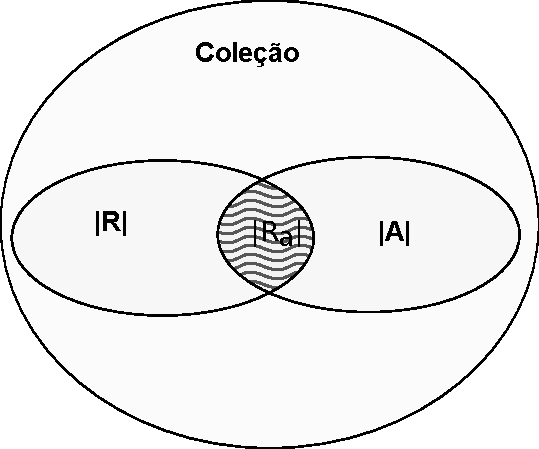
\includegraphics[width=3cm]{./recall.pdf}
    % recall.pdf: 259x216 pixel, 72dpi, 9.14x7.62 cm, bb=0 0 259 216
  \end{figure}
\column{4cm}
  \begin{equation*}
    Precis\tilde{a}o = \frac{|R_a|}{|A|}
  \end{equation*} 
\end{columns}
\end{frame}

\begin{frame}[fragile]
\frametitle{Problemas}
\begin{itemize}
 \item Conjunto $|R|$ em situações reais pode ser difícil ou impossível de determinar.
  \item 
\end{itemize}


\end{frame}

\end{document}
